\panel{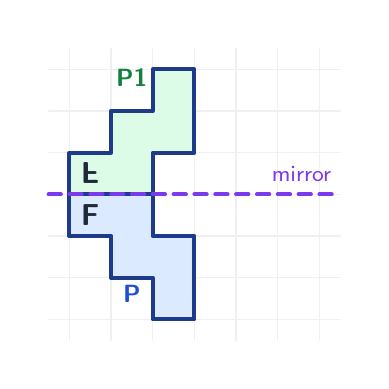
\begin{tikzpicture}[x=1bp, y=1bp]\path[use as bounding box] (0,0) rectangle (120.00,120.00);\clip (0,0) rectangle (120.00,120.00);
\path[draw={rgb,255:red,238;green,240;blue,243}, line width=0.52bp, line cap=round, line join=round] (15.00,7.50) -- (15.00,112.50);
\path[draw={rgb,255:red,238;green,240;blue,243}, line width=0.52bp, line cap=round, line join=round] (30.00,7.50) -- (30.00,112.50);
\path[draw={rgb,255:red,238;green,240;blue,243}, line width=0.52bp, line cap=round, line join=round] (45.00,7.50) -- (45.00,112.50);
\path[draw={rgb,255:red,238;green,240;blue,243}, line width=0.52bp, line cap=round, line join=round] (60.00,7.50) -- (60.00,112.50);
\path[draw={rgb,255:red,238;green,240;blue,243}, line width=0.52bp, line cap=round, line join=round] (75.00,7.50) -- (75.00,112.50);
\path[draw={rgb,255:red,238;green,240;blue,243}, line width=0.52bp, line cap=round, line join=round] (90.00,7.50) -- (90.00,112.50);
\path[draw={rgb,255:red,238;green,240;blue,243}, line width=0.52bp, line cap=round, line join=round] (105.00,7.50) -- (105.00,112.50);
\path[draw={rgb,255:red,238;green,240;blue,243}, line width=0.52bp, line cap=round, line join=round] (7.50,15.00) -- (112.50,15.00);
\path[draw={rgb,255:red,238;green,240;blue,243}, line width=0.52bp, line cap=round, line join=round] (7.50,30.00) -- (112.50,30.00);
\path[draw={rgb,255:red,238;green,240;blue,243}, line width=0.52bp, line cap=round, line join=round] (7.50,45.00) -- (112.50,45.00);
\path[draw={rgb,255:red,238;green,240;blue,243}, line width=0.52bp, line cap=round, line join=round] (7.50,60.00) -- (112.50,60.00);
\path[draw={rgb,255:red,238;green,240;blue,243}, line width=0.52bp, line cap=round, line join=round] (7.50,75.00) -- (112.50,75.00);
\path[draw={rgb,255:red,238;green,240;blue,243}, line width=0.52bp, line cap=round, line join=round] (7.50,90.00) -- (112.50,90.00);
\path[draw={rgb,255:red,238;green,240;blue,243}, line width=0.52bp, line cap=round, line join=round] (7.50,105.00) -- (112.50,105.00);
\path[fill={rgb,255:red,219;green,234;blue,254}] (15.00,45.00) rectangle (30.00,60.00);
\path[fill={rgb,255:red,219;green,234;blue,254}] (30.00,45.00) rectangle (45.00,60.00);
\path[fill={rgb,255:red,219;green,234;blue,254}] (30.00,30.00) rectangle (45.00,45.00);
\path[fill={rgb,255:red,219;green,234;blue,254}] (45.00,30.00) rectangle (60.00,45.00);
\path[fill={rgb,255:red,219;green,234;blue,254}] (45.00,15.00) rectangle (60.00,30.00);
\path[fill={rgb,255:red,220;green,252;blue,231}] (15.00,60.00) rectangle (30.00,75.00);
\path[fill={rgb,255:red,220;green,252;blue,231}] (30.00,60.00) rectangle (45.00,75.00);
\path[fill={rgb,255:red,220;green,252;blue,231}] (30.00,75.00) rectangle (45.00,90.00);
\path[fill={rgb,255:red,220;green,252;blue,231}] (45.00,75.00) rectangle (60.00,90.00);
\path[fill={rgb,255:red,220;green,252;blue,231}] (45.00,90.00) rectangle (60.00,105.00);
\path[draw={rgb,255:red,30;green,58;blue,138}, line width=1.50bp, line join=round] (15.00,60.00) -- (45.00,60.00) -- (45.00,45.00) -- (60.00,45.00) -- (60.00,15.00) -- (45.00,15.00) -- (45.00,30.00) -- (30.00,30.00) -- (30.00,45.00) -- (15.00,45.00) -- cycle;
\path[draw={rgb,255:red,30;green,58;blue,138}, line width=1.50bp, line join=round] (15.00,60.00) -- (45.00,60.00) -- (45.00,75.00) -- (60.00,75.00) -- (60.00,105.00) -- (45.00,105.00) -- (45.00,90.00) -- (30.00,90.00) -- (30.00,75.00) -- (15.00,75.00) -- cycle;
\path[draw={rgb,255:red,124;green,58;blue,237}, line width=1.35bp, dash pattern=on 4.50bp off 3.00bp, line cap=round, line join=round] (7.50,60.00) -- (112.50,60.00);
\node[anchor=base east, text={rgb,255:red,124;green,58;blue,237}, font=\fontsize{7.9}{9.4}\selectfont\sffamily, inner sep=0pt] at (109.50,64.50) {mirror};
\node[anchor=base, text={rgb,255:red,21;green,128;blue,61}, font=\fontsize{9.0}{10.8}\selectfont\sffamily\bfseries, inner sep=0pt] at (37.50,99.00) {P1};
\begin{scope}[shift={(22.50,52.50)}, xscale=1, yscale=1]\node[transform shape, inner sep=0pt, text={rgb,255:red,31;green,41;blue,55}, font=\fontsize{11.2}{11.2}\selectfont\sffamily\bfseries] {F};\end{scope}
\begin{scope}[shift={(22.50,67.50)}, xscale=1, yscale=-1]\node[transform shape, inner sep=0pt, text={rgb,255:red,31;green,41;blue,55}, font=\fontsize{11.2}{11.2}\selectfont\sffamily\bfseries] {F};\end{scope}
\node[anchor=base, text={rgb,255:red,29;green,78;blue,216}, font=\fontsize{9.0}{10.8}\selectfont\sffamily\bfseries\itshape, inner sep=0pt] at (37.50,21.00) {P};
\end{tikzpicture}}{(a) $P$1: reflect across the $x$-axis}\hspace{30.0bp}\panel{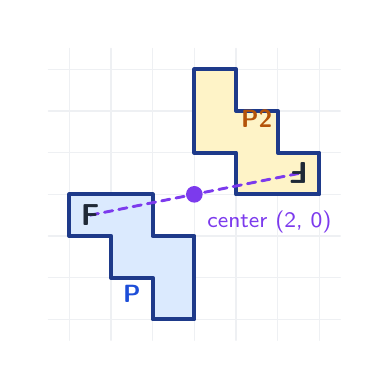
\begin{tikzpicture}[x=1bp, y=1bp]\path[use as bounding box] (0,0) rectangle (120.00,120.00);\clip (0,0) rectangle (120.00,120.00);
\path[draw={rgb,255:red,238;green,240;blue,243}, line width=0.52bp, line cap=round, line join=round] (15.00,7.50) -- (15.00,112.50);
\path[draw={rgb,255:red,238;green,240;blue,243}, line width=0.52bp, line cap=round, line join=round] (30.00,7.50) -- (30.00,112.50);
\path[draw={rgb,255:red,238;green,240;blue,243}, line width=0.52bp, line cap=round, line join=round] (45.00,7.50) -- (45.00,112.50);
\path[draw={rgb,255:red,238;green,240;blue,243}, line width=0.52bp, line cap=round, line join=round] (60.00,7.50) -- (60.00,112.50);
\path[draw={rgb,255:red,238;green,240;blue,243}, line width=0.52bp, line cap=round, line join=round] (75.00,7.50) -- (75.00,112.50);
\path[draw={rgb,255:red,238;green,240;blue,243}, line width=0.52bp, line cap=round, line join=round] (90.00,7.50) -- (90.00,112.50);
\path[draw={rgb,255:red,238;green,240;blue,243}, line width=0.52bp, line cap=round, line join=round] (105.00,7.50) -- (105.00,112.50);
\path[draw={rgb,255:red,238;green,240;blue,243}, line width=0.52bp, line cap=round, line join=round] (7.50,15.00) -- (112.50,15.00);
\path[draw={rgb,255:red,238;green,240;blue,243}, line width=0.52bp, line cap=round, line join=round] (7.50,30.00) -- (112.50,30.00);
\path[draw={rgb,255:red,238;green,240;blue,243}, line width=0.52bp, line cap=round, line join=round] (7.50,45.00) -- (112.50,45.00);
\path[draw={rgb,255:red,238;green,240;blue,243}, line width=0.52bp, line cap=round, line join=round] (7.50,60.00) -- (112.50,60.00);
\path[draw={rgb,255:red,238;green,240;blue,243}, line width=0.52bp, line cap=round, line join=round] (7.50,75.00) -- (112.50,75.00);
\path[draw={rgb,255:red,238;green,240;blue,243}, line width=0.52bp, line cap=round, line join=round] (7.50,90.00) -- (112.50,90.00);
\path[draw={rgb,255:red,238;green,240;blue,243}, line width=0.52bp, line cap=round, line join=round] (7.50,105.00) -- (112.50,105.00);
\path[fill={rgb,255:red,219;green,234;blue,254}] (15.00,45.00) rectangle (30.00,60.00);
\path[fill={rgb,255:red,219;green,234;blue,254}] (30.00,45.00) rectangle (45.00,60.00);
\path[fill={rgb,255:red,219;green,234;blue,254}] (30.00,30.00) rectangle (45.00,45.00);
\path[fill={rgb,255:red,219;green,234;blue,254}] (45.00,30.00) rectangle (60.00,45.00);
\path[fill={rgb,255:red,219;green,234;blue,254}] (45.00,15.00) rectangle (60.00,30.00);
\path[fill={rgb,255:red,254;green,243;blue,199}] (90.00,60.00) rectangle (105.00,75.00);
\path[fill={rgb,255:red,254;green,243;blue,199}] (75.00,60.00) rectangle (90.00,75.00);
\path[fill={rgb,255:red,254;green,243;blue,199}] (75.00,75.00) rectangle (90.00,90.00);
\path[fill={rgb,255:red,254;green,243;blue,199}] (60.00,75.00) rectangle (75.00,90.00);
\path[fill={rgb,255:red,254;green,243;blue,199}] (60.00,90.00) rectangle (75.00,105.00);
\path[draw={rgb,255:red,30;green,58;blue,138}, line width=1.50bp, line join=round] (15.00,60.00) -- (45.00,60.00) -- (45.00,45.00) -- (60.00,45.00) -- (60.00,15.00) -- (45.00,15.00) -- (45.00,30.00) -- (30.00,30.00) -- (30.00,45.00) -- (15.00,45.00) -- cycle;
\path[draw={rgb,255:red,30;green,58;blue,138}, line width=1.50bp, line join=round] (105.00,60.00) -- (75.00,60.00) -- (75.00,75.00) -- (60.00,75.00) -- (60.00,105.00) -- (75.00,105.00) -- (75.00,90.00) -- (90.00,90.00) -- (90.00,75.00) -- (105.00,75.00) -- cycle;
\path[draw={rgb,255:red,124;green,58;blue,237}, line width=1.05bp, dash pattern=on 3.00bp off 2.25bp, line cap=round, line join=round] (22.50,52.50) -- (97.50,67.50);
\path[fill={rgb,255:red,124;green,58;blue,237}] (60.00,60.00) circle[radius=3.00bp];
\node[anchor=base west, text={rgb,255:red,124;green,58;blue,237}, font=\fontsize{7.9}{9.4}\selectfont\sffamily, inner sep=0pt] at (64.50,48.00) {center (2, 0)};
\node[anchor=base, text={rgb,255:red,180;green,83;blue,9}, font=\fontsize{9.0}{10.8}\selectfont\sffamily\bfseries, inner sep=0pt] at (82.50,84.00) {P2};
\begin{scope}[shift={(22.50,52.50)}, xscale=1, yscale=1]\node[transform shape, inner sep=0pt, text={rgb,255:red,31;green,41;blue,55}, font=\fontsize{11.2}{11.2}\selectfont\sffamily\bfseries] {F};\end{scope}
\begin{scope}[shift={(97.50,67.50)}, xscale=-1, yscale=-1]\node[transform shape, inner sep=0pt, text={rgb,255:red,31;green,41;blue,55}, font=\fontsize{11.2}{11.2}\selectfont\sffamily\bfseries] {F};\end{scope}
\node[anchor=base, text={rgb,255:red,29;green,78;blue,216}, font=\fontsize{9.0}{10.8}\selectfont\sffamily\bfseries\itshape, inner sep=0pt] at (37.50,21.00) {P};
\end{tikzpicture}}{(b) $P$2: a half turn around (2,~0)}
